\documentclass{article}
\usepackage[T1]{fontenc}
\usepackage{lmodern}
\usepackage{graphicx}
\usepackage{amsmath,amssymb}
\usepackage[a4paper,margin=2cm]{geometry}
\usepackage[absolute,overlay]{textpos}
\setlength{\TPHorizModule}{1mm}
\setlength{\TPVertModule}{1mm}
\usepackage[indonesian]{babel}
\usepackage{hyperref}
\setlength{\emergencystretch}{2em}
% unit: Halaman 16

\begin{document}

% === Halaman 16 (llm) ===

\begin{itemize}
  \item Mula-mula, semua \textit{byte} dari kunci eksternal, $K[0..b-1]$, disalin ke dalam larik $L$ yang berukuran $c$ \textit{word}, $L[0..c-1]$. (ingat: $b$ dalam byte, $c$ dalam word, $c < b$)
  \item lalu \textit{padding} dengan sejumlah 0 jika perlu (\textit{padding} terjadi jika $b$ bukan kelipatan $w$).
  \item Kemudian inisialisasi larik S sebagai berikut:
\end{itemize}

\begin{align*}
S[0] \leftarrow P_w \\
\textbf{for } i \leftarrow 1 \text{ to } t-1 \textbf{ do} \\
\quad S[i] \leftarrow S[i-1] + Q_w \\
\textbf{endfor}
\end{align*}

\vspace{10mm}

% deskripsi: Tabel parameter yang berisi kolom Parameter, Simbol, dan Nilai yang dibolehkan untuk w, r, dan b.
% bbox normalisasi: [0.4010, 0.5700, 0.9810, 0.7920]
\begin{textblock*}{121.80mm}(84.21mm,169.29mm)
\noindent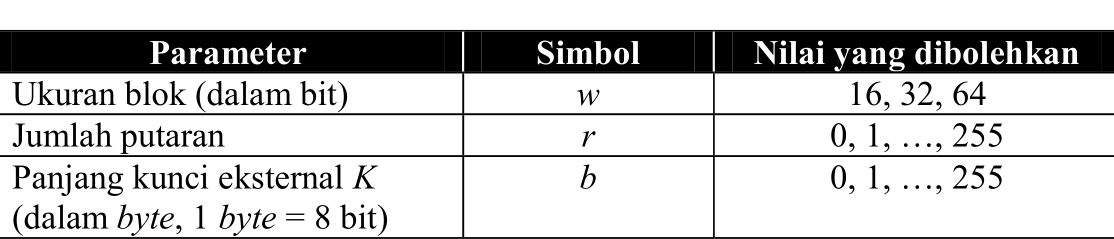
\includegraphics[width=121.80mm,height=65.93mm]{../../images/llm/page_016_img_01.png}%
\end{textblock*}

\end{document}
